\hsection{Inheritance}%
\label{sec:inheritance}%
%
\hsection{A Hierarchy of Geometric Objects}%
%
\begin{figure}[tb]%
\centering%
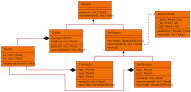
\includegraphics[width=0.985\linewidth]{\currentDir/exampleInheritance}%
\caption{An example for class inheritance. %
The base class \pythonil{Shape} offers two abstract methods, \pythonil{area} and \pythonil{perimeter}. %
The class \pythonil{Circle} inherits from \pythonil{Shape} and implements these methods. %
It also has an attribute \pythonil{center}, which is an instance of~\pythonil{Point}, and an attribute~\pythonil{radius}. %
The class \pythonil{Polygon} extends \pythonil{Shape} as well, and offers, amongst others, an \pythonilIdx{Iterable} of its~\pythonils{Point}. %
It also uses our \pythonil{KahanSum} to implement the \pythonil{perimeter} method. %
The class \pythonil{Polygon} is realized by the classes \pythonil{Triangle} and \pythonil{Rectangle}.}%
\label{fig:exampleInheritance}%
\end{figure}%
%
\gitPython{\programmingWithPythonCodeRepo}{classes/shape.py}{--args format}{classes:shape}{%
A class for representing shapes in the two-dimensional Euclidean plane.}%
%
\gitPython{\programmingWithPythonCodeRepo}{classes/circle.py}{--args format}{classes:circle}{%
A circle is a special shape, namely the set of all points whose distance from the center of the circle is exactly the radius.}%
%
\gitPythonAndOutput{\programmingWithPythonCodeRepo}{classes}{circle_user.py}{--args format}{classes:circle_user}{%
An example of using our class \pythonil{Circle} from \cref{lst:classes:circle}.}%
%
\gitPython{\programmingWithPythonCodeRepo}{classes/polygon.py}{--args format}{classes:polygon}{%
Polygons are special shapes delimited by straight lines between corner points.}%
%
\gitPython{\programmingWithPythonCodeRepo}{classes/rectangle.py}{--args format}{classes:rectangle}{%
Two different points in a plane span a rectangle, which is a special polygon.}%
%
\gitPython{\programmingWithPythonCodeRepo}{classes/triangle.py}{--args format}{classes:triangle}{%
A triangle is a polygon spanned by three points in a plane.}%
%
We already learned that classes are a proper tool four grouping data and operations on the data together into one semantic unit.
Classes also offer the concept of inheritance, which basically means \inQuotes{specialization}.
This concept is explored by a more elaborate example illustrated in \cref{fig:exampleInheritance}, which we will now discuss step-by-step.
Imagine that we would wanted to represent all geometrical shapes in a two-dimensional plane.
Each shape has an associated area as well as a perimeter.
We could create a class\pythonIdx{class} \pythonil{Shape} that provides two methods, \pythonil{area} and \pythonil{perimeter}, returning the area in in area units and the perimeter length in length units, respectively.

A circle is a special shape.
It does have a center as well as a radius.
Knowing these two attributes, we can compute the area and perimeter.
If we wanted to express this in terms of classes, we could say that the class\pythonIdx{class} \pythonil{Circle} is a special subclass of class~\pythonil{Shape}.
It would have two attributes, \pythonil{center} (which could be an instance of \pythonil{Point}) and \pythonil{radius}, which would be a \pythonil{float}.
The methods \pythonil{area} and \pythonil{perimeter} could then be implemented appropriately and use these attributes.

This is already how inheritance works:
If we want that a new class\pythonIdx{class}~\pythonil{Circle} inherits from a class\pythonIdx{class}~\pythonil{Shape}, all we have to do is to write \pythonil{class Circle(Shape):} instead of just \pythonil{class Circle:} when declaring the new circle class\pythonIdx{class}.
Of course, we first need to create the class\pythonIdx{class}~\pythonil{Shape}.

We do this in \cref{lst:classes:shape}.
In this listing, we define \pythonil{Shape} as a new class\pythonIdx{class}.
We want that this class has two methods, \pythonil{area} and \pythonil{perimeter}.
The class\pythonIdx{class}~\pythonil{Shape} is not intended for being instantiated.
Instead, we just want it to be the base class\pythonIdx{class} for \inQuotes{special} shapes.
It does not have any attribute.
Of course, we cannot really compute the area or the perimeter of such an abstract object.
So both methods raise\pythonIdx{raise} an \pythonilIdx{NotImplementedError}.
If someone would like to actually instantiate \pythonil{Shape} by doing, say, \pythonil{s = Shape()} and then invoke \pythonil{s.perimeter()}, this would fail.

While \pythonil{Shape} itself is useless, it allows us to create different specialized subclasses that do implement \pythonil{area} and \pythonil{perimeter}.
The user of these classes could then treat all of these different subclasses in the same way, because all of them support the interface defined by~\pythonil{Shape}.

In \cref{lst:classes:circle}, we define the class\pythonIdx{class}~\pythonil{Circle}.
By writing \pythonil{class Circle(Shape)}\pythonIdx{class}, we declare it as a subclass\pythonIdx{class} of \pythonil{Shape}.
Its initializer \dunder{init}, we supply two parameters, \pythonil{center}, which is an instance of our class \pythonil{Point} from \cref{lst:classes:point}, and \pythonil{radius}, which can either be an \pythonil{int} or a \pythonil{float}.
The initializer first checks if \pythonil{radius} is a finite and positive number.
Otherwise, it raises\pythonIdx{raise} a \pythonilIdx{ValueError}.
The initializer of the class\pythonIdx{class}~\pythonil{Point} already ensures that both coordinates of \pythonil{point} will be finite.
This ensures that we indeed create valid circles.
We store \pythonil{center} and \pythonil{radius} in two attributes of the same names.
We annotate them with the \pgls{typeHint} \pythonilIdx{Final}, which means that they should not be changed after the object is constructed.
We can now implement the function \pythonil{area} to return~$\numberPi\pythonil{radius}^2$ and \pythonil{perimeter} to return~$2\numberPi\pythonil{radius}$.
With this, the complete interface defined by the superclass\pythonIdx{class}~\pythonil{Shape} is now filled with meaning.

In \cref{lst:classes:circle_user}, we explore how this new class can be used.
We create the new instance \pythonil{circ} of \pythonil{Circle} by providing the \pythonil{point=Point(2, 3)} and \pythonil{radius=4}.
These parameters are indeed reflected by the corresponding attributes.
We also confirm that \pythonil{isinstance(cir, Circle)}\pythonIdx{isinstance} is \pythonil{True}.
It also holds that \pythonil{isinstance(cir, Shape)}\pythonIdx{isinstance}.
Every instance of \pythonil{Circle} is also an instance of \pythonil{Shape}.
Because \pythonil{Circle} is a special case of \pythonil{Shape}.

There are, of course, more shapes than just circles.
Another very general class of shapes are polygons.
Polygons are shapes enclosed by straight lines.
This means that every polygon can be defined by its corner points.
In \cref{lst:classes:polygon}, we define \pythonil{Polygon} as base class for such shapes.
It is a special case of (and thus inherits from)~\pythonil{Shape}.

\pythonil{Polygon} extends the interface of \pythonil{Shape} by offering the method~\pythonil{points}.
This method returns an \pythonilIdx{Iterable}\pythonIdx{typing.Iterable} of instances of~\pythonil{Point}, which are the corner points of the polygon.
Our goal here is to provide a base class for different types of \pythonils{Polygon}.
We do not actually want to implement a datastructure for arbitrary polygons here.
So the method \pythonil{points} raises\pythonIdx{raise} an \pythonil{NotImplementedError} and thus must be implemented by the subclasses that we will develop later.

If we know the sequence corner points and also know that they are connected by straight lines, then we can easily compute the perimeter of such a shape.
We can thus implement \pythonil{perimeter} as follows:
We iterate over the instances of~\pythonil{Point} returned by~\pythonil{points()}.
In a summation variable, we add up the distance between each point and its successor in the sequence.
Finally, we add the distance of the last point to the first point.
The distance can be computed with the \pythonil{distance} method offered by the \pythonil{Point} class.
While \pythonil{Polygon} itself does not implement \pythonil{points}, its subclasses will.
The method \pythonil{perimeter} will then \emph{automatically} use the actual implementation of the subclass.
We therefore can implement \pythonil{perimeter} here, even if \pythonil{points} is not yet implemented.
If we create a subclass that does implement \pythonil{points} and call \pythonil{perimeter} upon an instance of this subclass, it will work.

The summation could be easily done with a normal variable of type~\pythonil{float}.
However, since we implemented the  second-order \citeauthor{K1965PFRORTE}-\citeauthor{B1968NSIMA}-\citeauthor{N1974REVZSES} summation algorithm in~\cref{lst:classes:kahan_sum}, we instead use that one.
It should give us a very accurate result.
(Notice that we could not easily use~\pythonilIdx{fsum} here without first storing all distances in a list, because we need to add up over the sequence of points and also the distance from the last to the first point.
So our \pythonil{KahanSum} does have indeed some advantages.)
For convenience sake, we also add a method~\pythonil{print} to \pythonil{Polygon}, which just prints the sequence of points.

Rectangles and triangles are special cases of polygons.
We now implement them as classes \pythonil{Rectangle} and \pythonil{Triangle} in \cref{lst:classes:rectangle,lst:classes:triangle}, respectively, which both are subclasses of~\pythonil{Polygon}.

A rectangle can be defined using its bottom-left and top-right corner point.
In the initializer \dunder{init} of the class \pythonil{Rectangle}, we pass in two points~\pythonil{p1} and~\pythonil{p2}.
We raise\pythonIdx{raise} a \pythonilIdx{ValueError} if these would form an empty rectangle.
Otherwise, we store the minimum x\nobreakdashes-~and y\nobreakdashes-coordinate in the bottom-left point attribute~\pythonil{p1} and the maximum x\nobreakdashes-~and y\nobreakdashes-coordinate in the attribute~\pythonil{p2}, marking the top-right corner of our rectangle.

We implement the method \pythonil{points} to return all four corners of the rectangle.
We only needed to store two of them, but we here need to return all four to comply with the definition of the method as given in class~\pythonil{Polygon}.

The area of the rectangle is easily computed.
While we already inherit a perfectly fine method \pythonil{perimeter} computing the perimeter of our rectangle from \pythonil{Polygon} we still override it.
This makes sense because we can compute the perimeter faster and more exactly by simply returning twice the sum of the length of the horizontal and vertical side length of our rectangle.
The inherited \pythonil{perimeter} method would instead iterate over all four points and compute Euclidean distances using~\pythonil{sqrt}, which is both slower and less accurate (especially if our coordinates would be~\pythonils{int}).

The class \pythonil{Triangle} is implemented in very much the same fashion.
This time, we need to store all three corner points (and also return all of them in the \pythonil{points}~method implementation).
There also is no better way for computing the perimeter than what \pythonil{Polygon} already provides, so we this time do not override~\pythonil{perimeter}.
The area computation is implemented using the formula~$A=x_1(y_2-y_3)+x_2(y_3-y_1)+x_3(y_1-y_2)$ you probably remember from high school maths.

Notice that both subclasses of \pythonil{Polygon} offer some \pglspl{doctest} in the \pglspl{docstring}.
While I needed to keep the \pglspl{docstring} short to be able to fit the listings on pages, these \pglspl{doctest} still are instructive for the user.%
\endhsection%
%
\hsection{Summary}%
In this section, we have discussed how inheritance of classes in \python\ works.
We used this knowledge to construct a hierarchy of geometric objects in the two-dimensional Euclidean plane.
While doing this, we saw how methods can be defined in an abstract way in a base class and then implemented and filled with life in a subclass.

What we have seen here, of course in a very abridged manner, is how complex \pglspl{API} can be constructed and implemented.
In a way, the class \pythonil{Shape} defined an interface for geometric objects.
This interface defined that each object shall support the two operations \pythonil{area()} and \pythonil{perimeter()}.
The class \pythonil{Circle} then implements this \pgls{API}, and so do the classes~\pythonil{Triangle} and~\pythonil{Rectangle}.

OK, that was a bit far-fetched.
But in reality, it actually could be a bit like this.

Imagine that you develop an \pgls{API} for creating graphics programmatically.
Your \pgls{API} would basically act as a blank canvas.
It would probably provide a method to draw a rectangle with certain coordinates in a certain color.
It would probably provide another method to draw a line of a certain width and color connecting two points.
You could define this as a class with (at least) two methods \pythonil{draw_line} and \pythonil{draw_rectangle}.
We could then go an implement these methods in a class in such a way that constructs an SVG graphic~\cite{DDGLMSWFJJ2011SVGSSE} in memory.
Another implementation could instead construct an Adobe~PDF~\cite{A2024WDPM,A2008P3DMPDFP1P1} graphic.
While doing this would be more complex and exceed the space that we can reasonable use for an example in this book, the principle of the approach would not be very different from what you have already learned here.%
\endhsection%
%
\FloatBarrier%
\endhsection%
